% !TEX program = pdflatex
\documentclass[3p,11pt]{elsarticle}
\usepackage{amsmath,amssymb}
\usepackage{array}
\usepackage{booktabs}
\usepackage[tableposition=top]{caption}
\usepackage{enumitem}
\usepackage{tikz}
\usepackage{pgfplots}
\pgfplotsset{compat=1.18}
\usepackage{url}
\urlstyle{same}
\usepackage[hidelinks]{hyperref}
\emergencystretch=3em
% first-page footer: the page number alone
\makeatletter
\def\ps@pprintTitle{\let\@oddhead\@empty\let\@evenhead\@empty
  \def\@oddfoot{\hfil\thepage\hfil}\let\@evenfoot\@oddfoot}
\makeatother

% ---- notation ---------------------------------------------------------------
\newcommand{\kms}{km\,s$^{-1}$}
\newcommand{\mJyb}{mJy\,beam$^{-1}$}
\newcommand{\lnu}{erg\,s$^{-1}$\,Hz$^{-1}$}
\newcommand{\sci}[2]{#1\times10^{#2}}
\newcommand{\Msun}{M_\odot}
\newcommand{\Rsun}{R_\odot}

\begin{document}

\begin{frontmatter}

\title{Circularly polarised 144\,MHz emission from the radio-flaring triple b~Persei}

\author{Charles C. Norton}

\begin{abstract}
b~Persei (HD~26961, A1\,III, $117$\,pc) has been known as a radio source since 1973, a triple whose inner
pair is an ellipsoidal variable on a $1.53$\,d orbit and whose flares at gigahertz
frequencies are non-thermal. The third data release of the LOFAR Two-metre Sky Survey
holds a $144$\,MHz component $0.3''$ from the star, and its per-pointing Stokes~V images
of four epochs from 2016 to 2022 give $+0.44\pm0.09$\,\mJyb\ at the star's position
($5.1\sigma$), consistent between epochs; on 2018 November 21 Stokes~I and~V stand at
$0.75\pm0.15$ and $+0.68\pm0.15$\,\mJyb, a circularly polarised fraction of
$0.91\pm0.27$. Among the $204$ magnetic chemically peculiar stars of the Renson and
Manfroid catalogue within $300$\,pc that the images cover, b~Per is the only one above
$4\sigma$, and none of $816$ positions $22.5''$ away reaches it. The source's spectral
luminosity, $\sci{1.2}{16}$\,\lnu, and its brightness temperature, above
$\sci{1.6}{11}$\,K for any region smaller than the inner orbit, require coherent
emission. TESS gives the inner orbit's period as $1.5273435$\,d, and the four epochs
cover the orbit from phase $0.45$ through $0.12$ with Stokes~V positive in each. Gaia's velocity amplitude
puts the inner companion above $0.35\,\Msun$, and the ROSAT source on the system,
$\sci{7.2}{30}$\,erg\,s$^{-1}$, is $20$ to $140$ times the saturated X-ray output of a
main-sequence star of that mass. The emission reads as the electron-cyclotron maser of an
active, evolved companion locked to the orbit, as in Algol and RS~CVn binaries, with the
A star's own magnetosphere as the alternative its classification as an Si star allows.
\end{abstract}

\begin{keyword}
Radio continuum: stars \sep Stars: individual: b~Persei \sep Binaries: close \sep
Stars: activity \sep Masers \sep Polarization
\end{keyword}

\end{frontmatter}

% =============================================================================
\section{Introduction}\label{sec:intro}
% =============================================================================

Radio emission from close binaries with a cool, tidally locked active component has been
studied at gigahertz frequencies since the 1970s, when b~Persei was found as an
intermittent $8.085$\,GHz source~\cite{HjellmingWade1973} and shown to be a triple with
weak, non-periodic, non-thermal flares~\cite{Hill1976}. At $144$\,MHz, LOFAR hears active
stars by their coherent emission, strongly circularly polarised: active M
dwarfs~\cite{Callingham2021} and RS~CVn binaries~\cite{Toet2021}, catalogued over a
quarter of the northern sky by the circularly polarised survey of LOFAR's second data
release (V-LoTSS)~\cite{Callingham2023}. Two magnetic chemically peculiar stars were
detected there in total intensity, with circular polarisation below $60$ per
cent~\cite{Hajduk2022}.

The third data release of the LOFAR Two-metre Sky Survey (LoTSS-DR3) covers $88$ per
cent of the northern sky and publishes a Stokes~V image of each pointing's
epoch~\cite{Shimwell2026}. A measurement of those images at the magnetic chemically
peculiar stars and the planet hosts of the northern sky found one star above $4\sigma$,
b~Per, which lies outside V-LoTSS's sky. This note reports b~Per at $144$\,MHz over the
four DR3 epochs that cover it, with its inner orbit from TESS and the other bands'
archival data.

\subsection{Contributions}
\begin{enumerate}[leftmargin=*,itemsep=1pt]
\item The first detection of b~Per at $144$\,MHz: a LoTSS-DR3 component on the star and
circularly polarised emission in its per-pointing images, $5.1\sigma$ over four epochs
and a fraction near one in the brightest.
\item The inner orbit's ephemeris from three TESS sectors of 2019--2024, the orbital phases
of the four epochs, the companion's minimum mass from Gaia's velocity amplitude, and the
system's X-ray luminosity set against what such a companion can emit.
\end{enumerate}

% =============================================================================
\section{b Persei}\label{sec:star}
% =============================================================================

b~Per (HD~26961, HR~1324, HIP~20070) is a naked-eye A star of $V=4.6$, classified
A1\,III among spectroscopic binaries~\cite{Abt2009} and listed as an A2 Si star in the
catalogue of Ap, HgMn and Am stars~\cite{RensonManfroid2009}; studies of the rotation of
magnetic chemically peculiar stars include it~\cite{Netopil2017,Bernhard2020}, and no
measurement of its magnetic field is found in the literature. Its light varies as an
ellipsoidal variable~\cite{Stebbins1923}. Hill et al.\ found the triple: the A star with
an unseen companion on a $1.53$\,d orbit, and a third star on an orbit of about
$700$\,d~\cite{Hill1976}. Gaia DR3~\cite{Gaia2023} gives a parallax of
$8.547\pm0.233$\,mas ($117\pm3$\,pc), $G=4.58$, $G_\mathrm{BP}-G_\mathrm{RP}=0.13$, a
renormalised unit weight error of $2.74$, and a robust radial-velocity amplitude of
$68.1$\,\kms\ over $41$ transits; with $K_1=34.1$\,\kms\ on the $1.527$\,d orbit the mass
function is $0.0063\,\Msun$, and for an A star of $2.3\,\Msun$ the companion's mass is at
least $0.35\,\Msun$. The ROSAT All-Sky Survey's bright-source catalogue~\cite{Voges1999}
holds 1RXS~J041814.8+501747, $4.2''$ from the star within its $7''$ error, at
$0.469\pm0.031$\,counts\,s$^{-1}$ and a hardness ratio HR1 of $0.19\pm0.06$, and the star
is among the A stars of that survey whose X-rays Schr\"oder and Schmitt
studied~\cite{SchroderSchmitt2007}. It is one of the radio stars observed to link the
Hipparcos frame to the radio frame~\cite{Walter1997}.

% =============================================================================
\section{Data and method}\label{sec:method}
% =============================================================================

\paragraph{LoTSS-DR3} Each DR3 pointing is an $8$\,h observation of one epoch. The
ASTRON VO's table of DR3 pointings gives the midpoint of each observation, and the SURF
Data Repository holds each pointing's products as tar archives, from which the $6''$
dirty Stokes~I and V planes were read by HTTP byte range, a patch around the star alone,
and put on DR3's flux scale by the factor the release gives for the pointing. The search
that found b~Per measured Stokes~V at the Si, Sr, Cr, Eu and He-peculiar stars of the
Renson and Manfroid catalogue north of $-1^\circ$ within $300$\,pc and at the NASA
Exoplanet Archive's hosts within $100$\,pc, each star carried to the pointing's epoch in
its two nearest pointings, its noise from the robust scatter of the annulus $12''$--$30''$
out, positions $22.5''$ away serving as the null: $204$ peculiar stars at a median
$5\sigma$ limit of $0.53$\,\mJyb\ and $353$ hosts at $0.49$\,\mJyb. For b~Per every
pointing within $3^\circ$ was read, with positions $1'$ north and south as controls, and
the source density of its field was counted in a $10'$ patch of its brightest epoch,
local maxima above $4\sigma$ with the star excluded.

\paragraph{TESS} The two-minute PDCSAP light curves of sectors 19, 59 and 86
(2019--2024), $44685$ cadences of quality zero, each normalised to its median, were
fitted with the inner orbit's frequency and its first two harmonics and one level and
slope per sector over a fine grid of periods, the period's error from the curvature of
$\chi^2$ with the residual scatter as the noise. Sector~59 carries the slow drifts of a
saturated star's photometry, and the shape of the curve is read from sector~19. The
ephemeris for phases places phase zero at the deeper minimum.

\paragraph{Other bands} The VLA Sky Survey's quick-look images of three epochs were
read at the Canadian Astronomy Data Centre, the brightest pixel within $2.5''$ of the
star's position at each date against the image noise and against the same statistic at
$2000$ random positions $15''$--$150''$ away. The ROSAT count rate is converted to flux
in $0.1$--$2.4$\,keV with the hardness-dependent factor of Schmitt et
al.~\cite{Schmitt1995}.

% =============================================================================
\section{Results}\label{sec:results}
% =============================================================================

\subsection{The 144 MHz source}

The DR3 catalogue holds ILTJ041814.68+501742.5, of peak $0.42\pm0.08$\,\mJyb\ and
integrated $0.79\pm0.22$\,mJy, $0.3''$ from the star's position at DR3's mean epoch. In
the star's own field the images hold $394$ sources per square degree at least as bright
as the star's, so a source falls within $1.5''$ of a given position by chance with
probability $\sci{2.1}{-4}$. In the search, b~Per is the only one of the $204$ peculiar
stars above $4\sigma$ in Stokes~V, and none of the $816$ positions $22.5''$ from them
reaches $4\sigma$.

\begin{table}[t]
\centering\small
\caption{b~Per in the per-pointing images of LoTSS-DR3: the pointing, the date of the
observation's midpoint, the star's distance from the pointing centre, DR3's flux-scale
factor, the phase range of the $8$\,h observation on the TESS ephemeris of the inner
orbit, the dirty Stokes~I peak within $4.5''$ of the star and its offset, and Stokes~V at
that peak and at the star's position, all on DR3's flux scale.}
\label{tab:lofar}
\setlength{\tabcolsep}{4.5pt}
\begin{tabular}{llrrcrrrr}
\toprule
Pointing & Date & Offset ($^\circ$) & Scale & Phase & $I$ (\mJyb) & ($''$) & $V_\mathrm{peak}$ & $V_\mathrm{star}$ \\
\midrule
P063+52 & 2016 Nov 10 & $1.42$ & $0.957$ & $0.75$--$0.97$ & $0.12\pm0.15$ & $4.5$ & $+0.42$ & $+0.31\pm0.14$ \\
P063+49 & 2018 Nov 21 & $1.44$ & $1.027$ & $0.90$--$0.12$ & $0.75\pm0.15$ & $0.0$ & $+0.68$ & $+0.68\pm0.15$ \\
P067+49 & 2018 Dec 1 & $2.24$ & $1.021$ & $0.45$--$0.67$ & $1.04\pm0.29$ & $1.5$ & $+0.26$ & $+0.24\pm0.21$ \\
P067+52 & 2022 May 7 & $2.31$ & $1.053$ & $0.53$--$0.75$ & $0.80\pm0.33$ & $4.5$ & $-0.09$ & $+0.45\pm0.30$ \\
\bottomrule
\end{tabular}
\end{table}

Table~\ref{tab:lofar} gives the four epochs. On 2018 November 21 the dirty images hold a
Stokes~I peak of $0.75\pm0.15$\,\mJyb\ on the star and Stokes~V of $+0.68\pm0.15$\,\mJyb\
there, a circularly polarised fraction of $0.91\pm0.27$. Ten days later Stokes~I reaches
$1.04\pm0.29$\,\mJyb\ $1.5''$ from the star, with Stokes~V of $+0.24\pm0.21$\,\mJyb\ at the
star's position; in 2016 and 2022 Stokes~I stands below $3\sigma$ and Stokes~V at
$+0.31\pm0.14$ and $+0.45\pm0.30$\,\mJyb. Read at the star's position, the four epochs give
$+0.44\pm0.09$\,\mJyb\ ($5.1\sigma$), consistent with one value ($\chi^2=4.6$ for $3$
degrees of freedom), and the three without November 21 give $+0.31\pm0.11$\,\mJyb\
($2.8\sigma$). The eight control reads $1'$ north and south of the star stay within
$1.0\sigma$.

At $117$\,pc the November source has a spectral luminosity of $\sci{1.2}{16}$\,\lnu, and
the mean circularly polarised flux one of $\sci{7}{15}$\,\lnu. Emission confined to a
region the size of the inner orbit, $7.9\,\Rsun$ for the masses above, would have a
brightness temperature of $\sci{1.6}{11}$\,K, and one the size of a $0.55\,\Rsun$ star
$\sci{3}{13}$\,K.

\subsection{Other bands}

In the VLA Sky Survey's quick-look images the star's position holds $0.25$\,\mJyb\
($1.8\sigma$) on 2019 March 5, $0.71\pm0.21$\,\mJyb\ ($3.3\sigma$) $0.5''$ from it on 2021
November 13, a level random positions of the image reach in $1.4$ per cent of cases, and
$0.27$\,\mJyb\ ($2.1\sigma$) on 2024 May 25; NVSS at $1.4$\,GHz and TGSS at $150$\,MHz hold
nothing within $30''$, at limits of a few and about twenty millijanskys. The ROSAT rate
gives $\sci{4.4}{-12}$\,erg\,cm$^{-2}$\,s$^{-1}$, an X-ray luminosity of
$\sci{7.2}{30}$\,erg\,s$^{-1}$. The G\"udel--Benz relation of active
stars~\cite{GudelBenz1993} pairs that luminosity with $\sci{2.3}{15}$\,\lnu\ at gigahertz
frequencies, $0.14$\,mJy at the star's distance, below the survey's reach.

\subsection{The inner orbit}

The TESS fit gives a period of $1.5273435\pm0.0000002$\,d, with phase zero, the deeper
minimum, at BJD~$2459919.73857$. In sector~19 (Figure~\ref{fig:fold}) the curve is a
double wave $5.9$ per cent from peak to trough, with minima $3.34$ and $1.32$ per cent
below the mean at phases $0.00$ and $0.51$ and maxima $2.52$ and $2.00$ per cent above it
at $0.27$ and $0.74$. The harmonic at half the period holds at $2.31$--$2.34$ per cent in
all three sectors and the term at the period, which makes the minima unequal, at
$0.95$--$1.14$ per cent. The four LoTSS-DR3 epochs fall at phases $0.75$--$0.97$,
$0.90$--$0.12$, $0.45$--$0.67$ and $0.53$--$0.75$, and Stokes~V is positive in each, the
largest value at the conjunction of phase zero.

\begin{figure}[t]
\centering
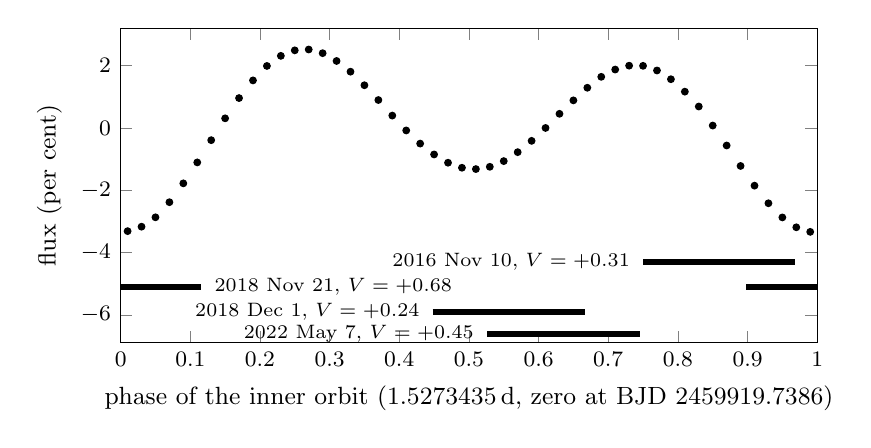
\begin{tikzpicture}
\begin{axis}[width=0.86\textwidth,height=0.46\textwidth,xmin=0,xmax=1,ymin=-6.9,ymax=3.2,
  xlabel={phase of the inner orbit ($1.5273435$\,d, zero at BJD 2459919.7386)},ylabel={flux (per cent)},
  tick label style={font=\footnotesize},label style={font=\small}]
\addplot[only marks,mark=*,mark size=1.2pt,black] coordinates {(0.01,-3.313) (0.03,-3.170) (0.05,-2.869) (0.07,-2.384) (0.09,-1.779) (0.11,-1.107) (0.13,-0.393) (0.15,0.308) (0.17,0.958) (0.19,1.525) (0.21,1.989) (0.23,2.313) (0.25,2.490) (0.27,2.517) (0.29,2.399) (0.31,2.149) (0.33,1.805) (0.35,1.370) (0.37,0.895) (0.39,0.396) (0.41,-0.081) (0.43,-0.503) (0.45,-0.851) (0.47,-1.117) (0.49,-1.278) (0.51,-1.321) (0.53,-1.248) (0.55,-1.065) (0.57,-0.778) (0.59,-0.415) (0.61,-0.001) (0.63,0.453) (0.65,0.884) (0.67,1.289) (0.69,1.640) (0.71,1.874) (0.73,1.998) (0.75,1.993) (0.77,1.844) (0.79,1.563) (0.81,1.164) (0.83,0.687) (0.85,0.076) (0.87,-0.564) (0.89,-1.221) (0.91,-1.853) (0.93,-2.418) (0.95,-2.873) (0.97,-3.190) (0.99,-3.336)};
\draw[black,line width=2.2pt] (axis cs:0.750,-4.3) -- (axis cs:0.968,-4.3);
\node[font=\scriptsize,anchor=east] at (axis cs:0.745,-4.3) {2016 Nov 10, $V=+0.31$};
\draw[black,line width=2.2pt] (axis cs:0.898,-5.1) -- (axis cs:1.0,-5.1);
\draw[black,line width=2.2pt] (axis cs:0.0,-5.1) -- (axis cs:0.116,-5.1);
\node[font=\scriptsize,anchor=west] at (axis cs:0.121,-5.1) {2018 Nov 21, $V=+0.68$};
\draw[black,line width=2.2pt] (axis cs:0.448,-5.9) -- (axis cs:0.666,-5.9);
\node[font=\scriptsize,anchor=east] at (axis cs:0.443,-5.9) {2018 Dec 1, $V=+0.24$};
\draw[black,line width=2.2pt] (axis cs:0.526,-6.6) -- (axis cs:0.745,-6.6);
\node[font=\scriptsize,anchor=east] at (axis cs:0.521,-6.6) {2022 May 7, $V=+0.45$};
\end{axis}
\end{tikzpicture}
\caption{The TESS light curve of b~Per in sector~19 (2019), folded on the ephemeris of
the inner orbit and binned in $50$ phase bins (errors smaller than the points); the bars
mark the phases each $8$\,h LoTSS-DR3 observation covered, with Stokes~V at the star's
position in \mJyb.}
\label{fig:fold}
\end{figure}

% =============================================================================
\section{Discussion}\label{sec:discussion}
% =============================================================================

A circularly polarised fraction near one and a brightness temperature above
$10^{11}$\,K for any region smaller than the inner orbit point to coherent emission, and
the electron-cyclotron maser is the coherent process a magnetised star sustains: at the
fundamental of the gyrofrequency $144$\,MHz needs about $51$\,G where it forms, at the
second harmonic about $26$\,G. The gigahertz emission of b~Per, non-thermal and
flaring~\cite{HjellmingWade1973,Hill1976}, and the X-ray source mark a magnetically
active component.

The X-ray luminosity places that component. A main-sequence star of $0.35$ to
$0.6\,\Msun$ emits at most about $10^{-3}$ of its bolometric luminosity in X-rays, $0.5$
to $\sci{3}{29}$\,erg\,s$^{-1}$, and the system's $\sci{7.2}{30}$\,erg\,s$^{-1}$ is $20$
to $140$ times that; A stars, without coronae or strong winds, emit far
less~\cite{SchroderSchmitt2007}. X-ray
luminosities of $10^{30}$ to $10^{31}$\,erg\,s$^{-1}$ belong to the evolved, tidally locked
active components of RS~CVn and Algol binaries, and in an Algol the low-mass companion of
an A or B star is a subgiant that has given up most of its mass. b~Per's inner companion
would then be such a star, locked to the $1.53$\,d orbit, and its magnetosphere the source
of the $144$\,MHz emission, as LOFAR hears in RS~CVn binaries~\cite{Toet2021}. The light
curve's term at the period, which keeps the minima unequal by about $1$ per cent in every
sector, fits a companion that contributes light and is lit by the A star. In the other
reading the A star, catalogued as an Si star~\cite{RensonManfroid2009}, carries a
magnetosphere whose electron-cyclotron maser is beamed across Earth, as in
CU~Vir~\cite{Trigilio2000}; synchronised to the orbit, its pulses would recur at fixed
orbital phases, while the four epochs show Stokes~V of one sign over two thirds of the
orbit.

Three measurements decide between the readings. The inner orbit spans $0.31$\,mas at the
star's distance, so very-long-baseline astrometry over one orbit places the radio
emission on one star or the other. A spectropolarimetric measurement of the A star's
longitudinal field would show whether it is magnetic. Time-resolved $144$\,MHz data, which
the DR3 visibilities hold, would show whether the emission comes in pulses at fixed phases
or varies as an active star's does. The A star 50~Cas carries a circularly polarised
$144$\,MHz source of the same kind with no companion above about $0.17\,\Msun$ on its
$1.6$\,d cycle~\cite{Norton2026}; b~Per shows such emission in a system whose active,
locked companion is known.

% =============================================================================
\section{Related work}\label{sec:related}
% =============================================================================

b~Per's radio emission was found at $8.085$\,GHz~\cite{HjellmingWade1973}, its flares and
triple nature described by Hill et al.~\cite{Hill1976}, and it was among the close
binaries of a centimetre-wave survey~\cite{Spangler1977} and the radio stars observed to
link the optical and radio reference frames~\cite{Walter1997}. At $144$\,MHz, V-LoTSS catalogued the
circularly polarised sources of LOFAR's second release~\cite{Callingham2023}, among them
RS~CVn binaries whose emission is coherent~\cite{Toet2021}, and the release's two magnetic
chemically peculiar stars are detections in total intensity~\cite{Hajduk2022}; neither
covers b~Per. No earlier detection of b~Per below $1$\,GHz is found in the literature.

% =============================================================================
\section{Conclusion}\label{sec:conclusion}
% =============================================================================

b~Per, a radio-flaring triple at $117$\,pc, carries a $144$\,MHz source in LoTSS-DR3,
circularly polarised at $+0.44\pm0.09$\,\mJyb\ over four epochs of 2016--2022 and at a
fraction near one in the brightest, at a luminosity of $\sci{1.2}{16}$\,\lnu\ and a
brightness temperature that requires coherent emission. Its inner orbit of
$1.5273435$\,d holds a companion of at least $0.35\,\Msun$, and its X-ray luminosity is
that of an evolved, locked active star rather than a dwarf, which makes that companion's
electron-cyclotron maser the reading the data favour; the A star's own magnetosphere is
the alternative, and astrometry of the radio source over one orbit would settle it.

\section*{Acknowledgements}

This work uses LoTSS-DR3 data from the LOFAR telescope, designed and constructed by
ASTRON, with its products served by the ASTRON VO and the SURF Data Repository; data
from the TESS mission, funded by NASA's Science Mission Directorate, obtained from the
Mikulski Archive for Space Telescopes; data from the European Space Agency mission
Gaia, processed by the Gaia Data Processing and Analysis Consortium, funded by national
institutions, in particular those participating in the Gaia Multilateral Agreement; the
VLA Sky Survey of the National Radio Astronomy Observatory, served by the Canadian
Astronomy Data Centre; the ROSAT All-Sky Survey, NVSS and TGSS catalogues; and the
SIMBAD and VizieR services at CDS, Strasbourg.

\begin{thebibliography}{99}\small\raggedright
\setlength{\itemsep}{1pt}

\bibitem{HjellmingWade1973}
R.~M. Hjellming and C.~M. Wade, Radio emission from the close binary b Persei,
\emph{Nature} \textbf{242}, 250 (1973).

\bibitem{Hill1976}
G.~Hill, G.~C.~L. Aikman, A.~P. Cowley, C.~T. Bolton and J.~C. Thomas, The radio-flaring
triple system b Per, \emph{Astrophys. J.} \textbf{208}, 152 (1976).

\bibitem{Callingham2021}
J.~R. Callingham, H.~K. Vedantham, T.~W. Shimwell, et al., The population of M dwarfs
observed at low radio frequencies, \emph{Nat. Astron.} \textbf{5}, 1233 (2021).

\bibitem{Toet2021}
S.~E.~B. Toet, H.~K. Vedantham, J.~R. Callingham, et al., Coherent radio emission from a
population of RS Canum Venaticorum systems, \emph{Astron. Astrophys.} \textbf{654}, A21
(2021).

\bibitem{Callingham2023}
J.~R. Callingham, T.~W. Shimwell, H.~K. Vedantham, et al., V-LoTSS: the circularly
polarised LOFAR Two-metre Sky Survey, \emph{Astron. Astrophys.} \textbf{670}, A124
(2023).

\bibitem{Hajduk2022}
M.~Hajduk, P.~Leto, H.~Vedantham, et al., Radio detection of chemically peculiar stars
with LOFAR, \emph{Astron. Astrophys.} \textbf{665}, A152 (2022).

\bibitem{Shimwell2026}
T.~W. Shimwell, M.~J. Hardcastle, C.~Tasse, et al., The LOFAR Two-metre Sky Survey: VII.
Third data release, \emph{Astron. Astrophys.} \textbf{707}, A198 (2026).

\bibitem{Abt2009}
H.~A. Abt, MK classifications of spectroscopic binaries, \emph{Astrophys. J. Suppl.}
\textbf{180}, 117 (2009).

\bibitem{RensonManfroid2009}
P.~Renson and J.~Manfroid, Catalogue of Ap, HgMn and Am stars, \emph{Astron. Astrophys.}
\textbf{498}, 961 (2009).

\bibitem{Netopil2017}
M.~Netopil, E.~Paunzen, S.~H\"ummerich and K.~Bernhard, An investigation of the rotational
properties of magnetic chemically peculiar stars, \emph{Mon. Not. R. Astron. Soc.}
\textbf{468}, 2745 (2017).

\bibitem{Bernhard2020}
K.~Bernhard, S.~H\"ummerich and E.~Paunzen, New and improved rotational periods of
magnetic CP stars from ASAS-3, KELT, and MASCARA data, \emph{Mon. Not. R. Astron. Soc.}
\textbf{493}, 3293 (2020).

\bibitem{Stebbins1923}
J.~Stebbins, The ellipsoidal variable star b Persei, \emph{Astrophys. J.} \textbf{57}, 1
(1923).

\bibitem{Gaia2023}
Gaia Collaboration, A.~Vallenari, A.~G.~A. Brown, et al., Gaia Data Release 3: summary
of the content and survey properties, \emph{Astron. Astrophys.} \textbf{674}, A1 (2023).

\bibitem{Voges1999}
W.~Voges, B.~Aschenbach, Th.~Boller, et al., The ROSAT all-sky survey bright source
catalogue, \emph{Astron. Astrophys.} \textbf{349}, 389 (1999).

\bibitem{SchroderSchmitt2007}
C.~Schr\"oder and J.~H.~M.~M. Schmitt, X-ray emission from A-type stars, \emph{Astron.
Astrophys.} \textbf{475}, 677 (2007).

\bibitem{Schmitt1995}
J.~H.~M.~M. Schmitt, T.~A. Fleming and M.~S. Giampapa, The X-ray view of the low-mass
stars in the solar neighborhood, \emph{Astrophys. J.} \textbf{450}, 392 (1995).

\bibitem{GudelBenz1993}
M.~G\"udel and A.~O. Benz, X-ray/microwave relation of different types of active stars,
\emph{Astrophys. J.} \textbf{405}, L63 (1993).

\bibitem{Trigilio2000}
C.~Trigilio, P.~Leto, F.~Leone, et al., Coherent radio emission from the magnetic
chemically peculiar star CU Virginis, \emph{Astron. Astrophys.} \textbf{362}, 281 (2000).

\bibitem{Norton2026}
C.~C. Norton, A variable, circularly polarised 144\,MHz source on the A2V star
50~Cassiopeiae, seti-tools \texttt{papers/hd12216} (2026).

\bibitem{Walter1997}
H.~G. Walter, R.~Hering and C.~de~Vegt, Radio stars for linking celestial reference
frames, \emph{Astron. Astrophys. Suppl.} \textbf{122}, 529 (1997).

\bibitem{Spangler1977}
S.~R. Spangler, F.~N. Owen and R.~A. Hulse, Radio survey of close binary stars,
\emph{Astron. J.} \textbf{82}, 989 (1977).

\end{thebibliography}

\end{document}
